% A LaTeX template for EXECUTIVE SUMMARY of the MSc Thesis submissions to 
% Politecnico di Milano (PoliMi) - School of Industrial and Information Engineering
%
% P. F. Antonietti, S. Bonetti, A. Gruttadauria, G. Mescolini, A. Zingaro
% e-mail: template-tesi-ingind@polimi.it
%
% Last Revision: October 2021
%
% Copyright 2021 Politecnico di Milano, Italy. Inc. All rights reserved.

\documentclass[10.5pt,a4paper,twocolumn]{article}

%------------------------------------------------------------------------------
%	REQUIRED PACKAGES AND  CONFIGURATIONS
%------------------------------------------------------------------------------
% PACKAGES FOR TITLES
\usepackage{titlesec}
\usepackage{color}

% PACKAGES FOR LANGUAGE AND FONT
\usepackage[utf8]{inputenc}
\usepackage[english]{babel}
\usepackage[T1]{fontenc} % Font encoding

% PACKAGES FOR IMAGES
\usepackage{graphicx}
\graphicspath{{Images/}} % Path for images' folder
\usepackage{eso-pic} % For the background picture on the title page
\usepackage{subfig} % Numbered and caption subfigures using \subfloat
\usepackage{caption} % Coloured captions
\usepackage{transparent}

% STANDARD MATH PACKAGES
\usepackage{amsmath}
\usepackage{amsthm}
\usepackage{bm}
\usepackage[overload]{empheq}  % For braced-style systems of equations

% PACKAGES FOR TABLES
\usepackage{tabularx}
\usepackage{longtable} % tables that can span several pages
\usepackage{colortbl}

% PACKAGES FOR ALGORITHMS (PSEUDO-CODE)
\usepackage{algorithm}
\usepackage{algorithmic}

% PACKAGES FOR REFERENCES & BIBLIOGRAPHY
\usepackage[colorlinks=true,linkcolor=black,anchorcolor=black,citecolor=black,filecolor=black,menucolor=black,runcolor=black,urlcolor=black]{hyperref} % Adds clickable links at references
\usepackage{cleveref}
\usepackage[square, numbers, sort&compress]{natbib} % Square brackets, citing references with numbers, citations sorted by appearance in the text and compressed
\bibliographystyle{plain} % You may use a different style adapted to your field

% PACKAGES FOR THE APPENDIX
\usepackage{appendix}

% PACKAGES FOR ITEMIZE & ENUMERATES 
\usepackage{enumitem}

% OTHER PACKAGES
\usepackage{amsthm,thmtools,xcolor} % Coloured "Theorem"
\usepackage{comment} % Comment part of code
\usepackage{fancyhdr} % Fancy headers and footers
\usepackage{lipsum} % Insert dummy text
\usepackage{tcolorbox} % Create coloured boxes (e.g. the one for the key-words)
\usepackage{stfloats} % Correct position of the tables

%-------------------------------------------------------------------------
%	NEW COMMANDS DEFINED
%-------------------------------------------------------------------------
% EXAMPLES OF NEW COMMANDS -> here you see how to define new commands
\newcommand{\bea}{\begin{eqnarray}} % Shortcut for equation arrays
\newcommand{\eea}{\end{eqnarray}}
\newcommand{\e}[1]{\times 10^{#1}}  % Powers of 10 notation
\newcommand{\mathbbm}[1]{\text{\usefont{U}{bbm}{m}{n}#1}} % From mathbbm.sty
\newcommand{\pdev}[2]{\frac{\partial#1}{\partial#2}}
% NB: you can also override some existing commands with the keyword \renewcommand

%----------------------------------------------------------------------------
%	ADD YOUR PACKAGES (be careful of package interaction)
%----------------------------------------------------------------------------


%----------------------------------------------------------------------------
%	ADD YOUR DEFINITIONS AND COMMANDS (be careful of existing commands)
%----------------------------------------------------------------------------


% Do not change Configuration_files/config.tex file unless you really know what you are doing. 
% This file ends the configuration procedures (e.g. customizing commands, definition of new commands)
% Set the geometric layout of the document
\usepackage{geometry}
\geometry{
  top=3cm,
  left = 2.0cm,
  right = 2.0cm,
  bottom=2cm,
  headheight= 2cm,
  headsep= 0cm,
}
\raggedbottom 

% Create color bluePoli (-> manuale grafica coordinata:  https://www.polimi.it/fileadmin/user_upload/il_Politecnico/grafica-coordinata/2015_05_11_46xy_manuale_grafica_coordinata.pdf)
\definecolor{bluePoli}{cmyk}{0.4,0.1,0,0.4}

% Custom theorem environments
\declaretheoremstyle[
  headfont=\color{bluePoli}\normalfont\bfseries,
  bodyfont=\color{black}\normalfont\itshape,
]{colored}

\captionsetup[figure]{labelfont={color=bluePoli}} % Set colour of the captions
\captionsetup[table]{labelfont={color=bluePoli}} % Set colour of the captions
\captionsetup[algorithm]{labelfont={color=bluePoli}} % Set colour of the captions

\theoremstyle{colored}
\newtheorem{theorem}{Theorem}[section]
\newtheorem{proposition}{Proposition}[section]

% Enhances the features of the standard "table" and "tabular" environments.
\newcommand\T{\rule{0pt}{2.6ex}}
\newcommand\B{\rule[-1.2ex]{0pt}{0pt}}

% Algorithm description
\newcounter{algsubstate}
\renewcommand{\thealgsubstate}{\alph{algsubstate}}
\newenvironment{algsubstates}{
    \setcounter{algsubstate}{0}%
    \renewcommand{\STATE}{%
    \stepcounter{algsubstate}%
    \Statex {\small\thealgsubstate:}\space}
    }{}
    
% Custom theorem environment
\newcolumntype{L}[1]{>{\raggedright\let\newline\\\arraybackslash\hspace{0pt}}m{#1}}
\newcolumntype{C}[1]{>{\centering\let\newline\\\arraybackslash\hspace{0pt}}m{#1}}
\newcolumntype{R}[1]{>{\raggedleft\let\newline\\\arraybackslash\hspace{0pt}}m{#1}}

% Custom itemize environment
\setlist[itemize,1]{label=$\bullet$}
\setlist[itemize,2]{label=$\circ$}
\setlist[itemize,3]{label=$-$}
\setlist{nosep}

% Set separation of columns 
\setlength{\columnsep}{30pt}

% Create command for background pic
\newcommand\BackgroundPic{% Adding background picture
	\put(230,358){
		\parbox[b][\paperheight]{\paperwidth}{%
			\vfill
			\centering
			\transparent{0.4}
			
\includegraphics[width=0.5\paperwidth]{raggiera_polimi.eps}%
			\vfill
}}}

% Set indentation
\setlength\parindent{0pt}

% Custom title commands
\titleformat{\section}
{\color{bluePoli}\normalfont\Large\bfseries}
{\color{bluePoli}\thesection.}{1em}{}
\titlespacing*{\section}
{0pt}{2ex}{1ex}

\titleformat{\subsection}
{\color{bluePoli}\normalfont\large\bfseries}
{\color{bluePoli}\thesubsection.}{1em}{}
\titlespacing*{\subsection}
{0pt}{2ex}{1ex}

% Custom headers and footers
\pagestyle{fancy}
\fancyhf{}
      
\fancyfoot{}
\fancyfoot[C]{\thepage} % page
\renewcommand{\headrulewidth}{0mm} % headrule width
\renewcommand{\footrulewidth}{0mm} % footrule width

\makeatletter
\patchcmd{\headrule}{\hrule}{\color{black}\hrule}{}{} % headrule
\patchcmd{\footrule}{\hrule}{\color{black}\hrule}{}{} % footrule
\makeatother

% -> Create the header
%\chead[C]{
%\centering
%\begin{tcolorbox}[arc=0pt, boxrule=0pt, colback=bluePoli!60, width=\textwidth, colupper=white]
%    \textbf{Executive summary} \hfill \textbf{\author}  
%\end{tcolorbox}
%}

% Insert here the info that will be displayed into your Title page 
% -> title of your work
\renewcommand{\title}{Homework 1: Image Classification}
% -> author name and surname
\renewcommand{\author}{ - Domenico Cacace \\  - Miguel Gonzalez \\  - Usevalad Milasheuski}
\renewcommand{\advisor}{DMU}


%-------------------------------------------------------------------------
%	BEGIN OF YOUR DOCUMENT
%-------------------------------------------------------------------------
\begin{document}

%-----------------------------------------------------------------------------
% TITLE PAGE
%-----------------------------------------------------------------------------
% Do not change Configuration_files/TitlePage.tex (Modify it IF AND ONLY IF you need to add or delete the Co-advisors)
% This file creates the Title Page of the document
% DO NOT REMOVE SPACES BETWEEN LINES!

\twocolumn[{\begin{@twocolumnfalse}

\AddToShipoutPicture*{\BackgroundPic}

\hspace{-0.6cm}
\includegraphics[width=0.6\textwidth]{logo_polimi_ing_indinf.eps}

\vspace{-1mm}
\fontsize{0.3cm}{0.5cm}\selectfont \bfseries \textsc{\color{bluePoli} Artificial Neural Networks and Deep Learning}\\

\vspace{-0.2cm}
\Large{\textbf{\color{bluePoli}{\title}}}\\

%\vspace{-0.2cm}
%\fontsize{0.3cm}{0.5cm}\selectfont \bfseries \textsc{\color{bluePoli} Laurea Magistrale in \course}\\

\vspace{-0.2cm}
\fontsize{0.3cm}{0.5cm} \selectfont \bfseries Authors: \\\textsc{\textbf{\author}}\\

\vspace{-0.4cm}
\fontsize{0.3cm}{0.5cm}\selectfont \bfseries Team name: \textsc{\textbf{\advisor}}\\


% if only ONE co-advisor is present:
%\vspace{-0.4cm}
%\fontsize{0.3cm}{0.5cm}\selectfont \bfseries Co-advisor: \textsc{\textbf{\firstcoadvisor}}\\
% if more than one co-advisors are present:
%\vspace{-0.4cm}
%\fontsize{0.3cm}{0.5cm}\selectfont \bfseries Co-advisors: \textsc{\textbf{\firstcoadvisor}}\textsc{\textbf{\secondcoadvisor}}\\

%\vspace{-0.4cm}
%\fontsize{0.3cm}{0.5cm}\selectfont \bfseries Academic year: \textsc{\textbf{\YEAR}}

\small \normalfont

%\vspace{11pt}

\centerline{\rule{1.0\textwidth}{0.4pt}}

\vspace{15pt}
\end{@twocolumnfalse}}]

\thispagestyle{plain} % In order to not show the header in the first page

%%%%%%%%%%%%%%%%%%%%%%%%%%%%%%
%%     THESIS MAIN TEXT     %%
%%%%%%%%%%%%%%%%%%%%%%%%%%%%%%

%-----------------------------------------------------------------------------
% INTRODUCTION
%-----------------------------------------------------------------------------
\section{Introduction}
\label{sec:introduction}
Our strategy for this homework is to start from a very simple model, and gradually analyze the results and make the adequate changes.
After reaching a \textit{decent} model made from scratch, we then jump to transfer learning, where we use a pre-trained network as a feature extractor, and train a classifier on top of it;
in the end, we compare our best models and draw our conclusions.

\section{Dataset}
\label{sec:dataset}
The dataset used in this project is a subset of PlantVillage.
Our dataset contains 17728 images of various plants, divided into 14 classes; 
the dataset was explicitly labeled (images of the same class are grouped in the corresponging subfolder, but it was not split in any way.
In order to correctly evaluate the model, we split the dataset into a training (80\%) and validation (20\%) set: 
to perform the split we first used the \texttt{ImageDataGenerator}'s \texttt{validation\_split} parameter, but in the end we used 
a \textit{manually} stratified split of the dataset, in order to cope with the different class distributions. 
We did not create a test set, as it was already provided on the CodaLab platform. 

All of the images are 3-channel RGB images, of size 256x256 pixels.

\section{First steps}
\label{sec:first_steps}
As a first step we built some small toy models, to evaluate on a small scale (without the need of waiting hours for the training to finish) which techniques worked best.
Our starting point was a simple model, with two convolutional layers (with MaxPooling), two dense layers and no particular technique: this model had a reasonable training accuracy,
but it was heavily overfitting the training set. To improve the model we added, step by step, dropout layers, regularization and data augmentation:
we observed how the validation accuracy improved with these techniques, but we were aware that the model was too simple to work.

In the following sections we actually tackle the classification problem; this means that we take the experimental results obtained on the toy model
and apply them (dropout, augmentation, regularization) on a real one. We also increase the batch size (256), the number of epochs (75-150) and add early stopping. 
Further details on the parameters used can be found in the model notebook.

\section{Our model, from scratch}
\label{sec:our_model}
Our first relevant\footnote{For the sake of brevity we omit models that, in our opinion, do not contribute significantly to the report} model was composed by 7 convolutional blocks and 2 dense layers; each convolutional block was composed by:
\begin{itemize}
    \item \texttt{Conv2D} layer, $3\times 3$ kernel, ReLU activation function
    \item \texttt{BatchNormalization} layer
    \item \texttt{Conv2D} layer, $3\times 3$ kernel, ReLU activation function
    \item \texttt{MaxPooling2D} layer, $2\times 2$ pooling, $2\times 2$ strides
\end{itemize}
We started with 8 filters in the first block, and doubled their number for each subsequent block, up to 512.
After the convolutional blocks we \texttt{Flatten} the output and add two dense (512, 14) layers.
With this model we scored 0.6792 on the test set, which is a decent baseline; the accuracy graph on the training and validation set are the following:
\begin{minipage}{0.5\textwidth}
    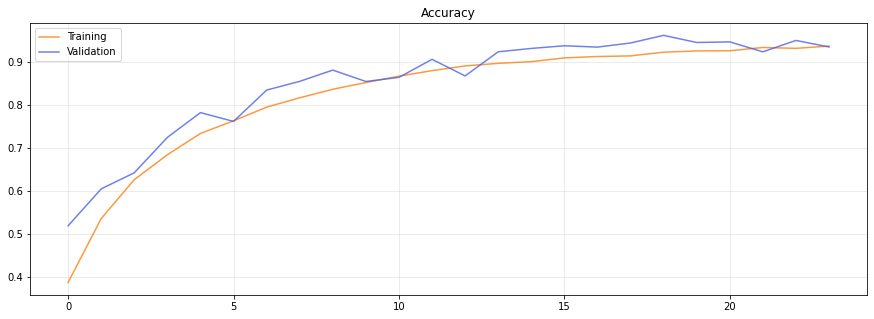
\includegraphics[width=\textwidth]{../graphs/accuracy/06_8conv2dense.png}
\end{minipage}

While finding a way to further improve our model we stumbled upon some articles suggesting that, 
following a similar idea to the one of data augmentation, we could add gaussian noise layers to increase the model robustness.
By adding two \texttt{GaussianNoise} layers, one after the first convolutional layer and the other before the output layer,
we obtained a 0.7302 on the test set, which is a good improvement.
\begin{minipage}{0.5\textwidth}
    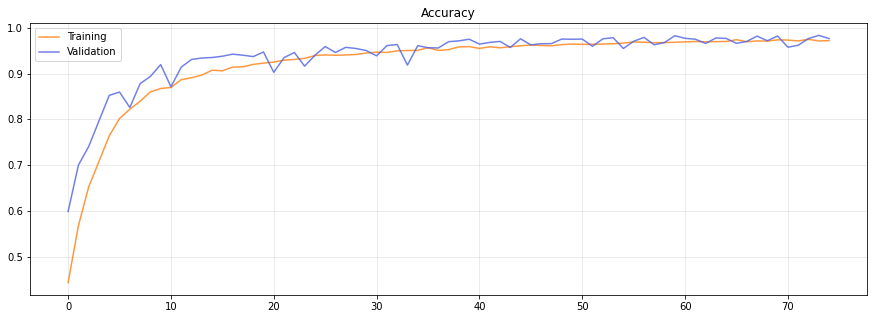
\includegraphics[width=\textwidth]{../graphs/accuracy.png}
    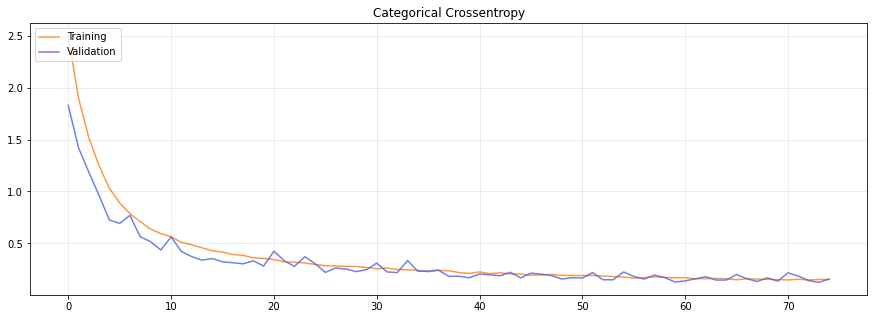
\includegraphics[width=\textwidth]{../graphs/crossentropy.png}
\end{minipage}


\section{Transfer learning}
\label{sec:transfer_learning}
We employed VGG16 with ImageNet weights as our feature extractor, and trained a classifier on top of it.

In a first moment we \textit{recycled} a previous MLP model, composed of
\begin{itemize}
    \item \texttt{Dense} layer, 512 neurons, ReLU activation function, dropout of 0.25
    \item \texttt{Dense} layer, 256 neurons, ReLU activation function, dropout of 0.25
    \item \texttt{Dense} layer (output), 14 neurons, softmax activation function
\end{itemize}
To connect the feature extractor with the classifier we used a \texttt{Flatten} layer, with dropout of 0.5.\\
This model achieves a validation accuracy of 0.9831, but its test accuracy is way lower (0.49): we ruled as a possible reason
for this behavior the scarcity of training data, so we implemented a data augmentation strategy to difersify the training set. 

By retraining the model with this tweak we ended up with the following accuracy graph:

\begin{minipage}{0.5\textwidth}
    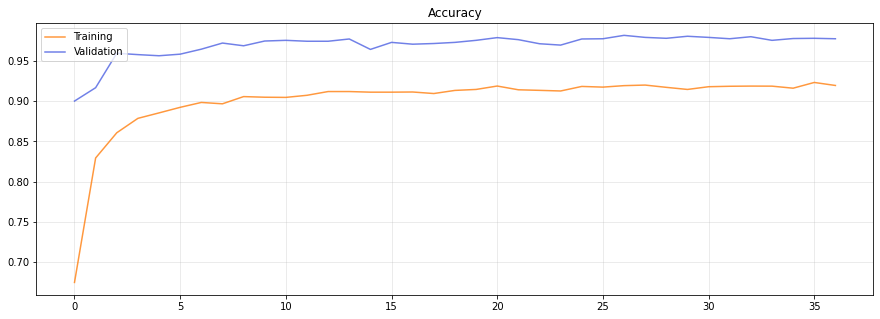
\includegraphics[width=\textwidth]{../graphs/accuracy/08_vgg16_aug.png}
\end{minipage}

As we can see, there is a significative gap between the training and validation accuracy: this can be attributed to the high dropout rates, 
that cause some neurons to shut down and having the subsequent layers trying to construct predictions based on incomplete data.
For this reason we ditched the dropout layers entirely, and observed that the gap tends to shrink.\\

Finally, to better suit VGG16 to our problem, we disabled the \texttt{freeze\_layer} parameter for the last convolutional block, in order to fine tune its weights.
The outcoming model scores 0.907 on the test set, and is our best model so far.
\begin{minipage}{0.5\textwidth}
    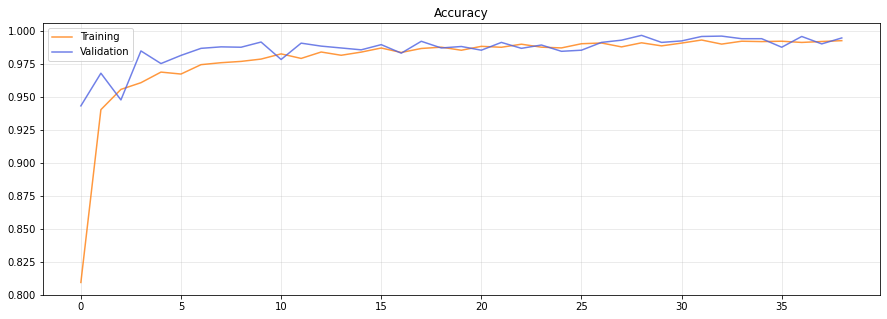
\includegraphics[width=\textwidth]{../graphs/accuracy/09_vgg16_aug_nodrop_finetune.png}
    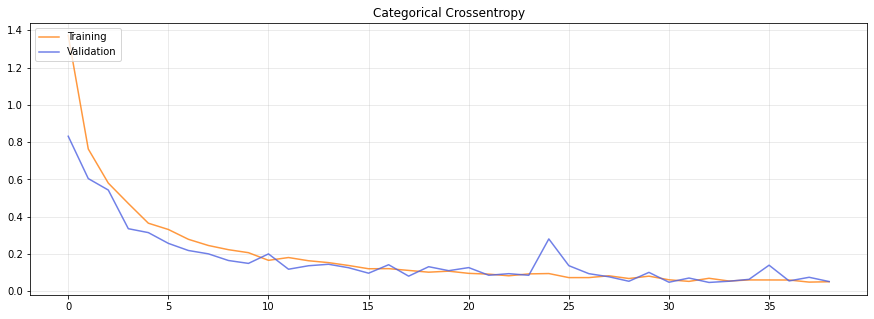
\includegraphics[width=\textwidth]{../graphs/categorical_crossentropy/09_vgg16_aug_nodrop_finetune.png}
\end{minipage}




%-----------------------------------------------------------------------------
% CONCLUSION
%-----------------------------------------------------------------------------
\section{Conclusions}
\label{sec:conclusions}
In conclusion we found that our best model, in terms of both accuracy and training time, was the last VGG16 model.
This however does not mean that transfer learning by itself is the panacea for all problems: as we could clearly see, 
just straight-up copying an existing model does not necessarily yield the best results, and knowing how to fine-tune it is a crucial step.


On a personal note, we are really happy with the results we achieved: it feels good to put in practice
the techniques learned during the theoretical lectures and to see how they can be applied to real problems.

\newpage
\onecolumn

\section{Appendix A: \textit{from scratch} model}
\begin{verbatim}
    Model: "sequential"
_________________________________________________________________
Layer (type)                 Output Shape              Param #   
=================================================================
conv2d (Conv2D)              (None, 256, 256, 8)       224       
_________________________________________________________________
batch_normalization (BatchNo (None, 256, 256, 8)       1024      
_________________________________________________________________
gaussian_noise (GaussianNois (None, 256, 256, 8)       0         
_________________________________________________________________
conv2d_1 (Conv2D)            (None, 256, 256, 8)       584       
_________________________________________________________________
max_pooling2d (MaxPooling2D) (None, 128, 128, 8)       0         
_________________________________________________________________
conv2d_2 (Conv2D)            (None, 128, 128, 16)      1168      
_________________________________________________________________
batch_normalization_1 (Batch (None, 128, 128, 16)      512       
_________________________________________________________________
conv2d_3 (Conv2D)            (None, 128, 128, 16)      2320      
_________________________________________________________________
max_pooling2d_1 (MaxPooling2 (None, 64, 64, 16)        0         
_________________________________________________________________
conv2d_4 (Conv2D)            (None, 64, 64, 32)        4640      
_________________________________________________________________
batch_normalization_2 (Batch (None, 64, 64, 32)        256       
_________________________________________________________________
conv2d_5 (Conv2D)            (None, 64, 64, 32)        9248      
_________________________________________________________________
max_pooling2d_2 (MaxPooling2 (None, 32, 32, 32)        0         
_________________________________________________________________
conv2d_6 (Conv2D)            (None, 32, 32, 64)        18496     
_________________________________________________________________
batch_normalization_3 (Batch (None, 32, 32, 64)        128       
_________________________________________________________________
conv2d_7 (Conv2D)            (None, 32, 32, 64)        36928     
_________________________________________________________________
max_pooling2d_3 (MaxPooling2 (None, 16, 16, 64)        0         
_________________________________________________________________
conv2d_8 (Conv2D)            (None, 16, 16, 128)       73856     
_________________________________________________________________
batch_normalization_4 (Batch (None, 16, 16, 128)       64        
_________________________________________________________________
conv2d_9 (Conv2D)            (None, 16, 16, 128)       147584    
_________________________________________________________________
max_pooling2d_4 (MaxPooling2 (None, 8, 8, 128)         0         
_________________________________________________________________
conv2d_10 (Conv2D)           (None, 8, 8, 256)         295168    
_________________________________________________________________
max_pooling2d_5 (MaxPooling2 (None, 4, 4, 256)         0         
_________________________________________________________________
flatten (Flatten)            (None, 4096)              0         
_________________________________________________________________
dropout (Dropout)            (None, 4096)              0         
_________________________________________________________________
dense (Dense)                (None, 512)               2097664   
_________________________________________________________________
dropout_1 (Dropout)          (None, 512)               0         
_________________________________________________________________
gaussian_noise_1 (GaussianNo (None, 512)               0         
_________________________________________________________________
dense_1 (Dense)              (None, 14)                7182      
=================================================================
Total params: 2,697,046
Trainable params: 2,696,054
Non-trainable params: 992
\end{verbatim}

\section{Appendix B: VGG16-based model}
\begin{verbatim}
    Model: "sequential"
_________________________________________________________________
Layer (type)                 Output Shape              Param #   
=================================================================
vgg16 (Functional)           (None, 8, 8, 512)         14714688  
_________________________________________________________________
flatten (Flatten)            (None, 32768)             0         
_________________________________________________________________
dense (Dense)                (None, 512)               16777728  
_________________________________________________________________
dense_1 (Dense)              (None, 256)               131328    
_________________________________________________________________
dense_2 (Dense)              (None, 14)                3598      
=================================================================
Total params: 31,627,342
Trainable params: 16,912,654
Non-trainable params: 14,714,688
_________________________________________________________________
\end{verbatim}

\end{document}